
\section{Engine Extensions}

Since most of the engine is very abstract in functionality, we have
made three extensions, which makes it easy to implement a tile based
environment, communicating with EIS supported APLs and log events.


\subsection{Tile Extension}

\begin{figure}
\begin{centering}
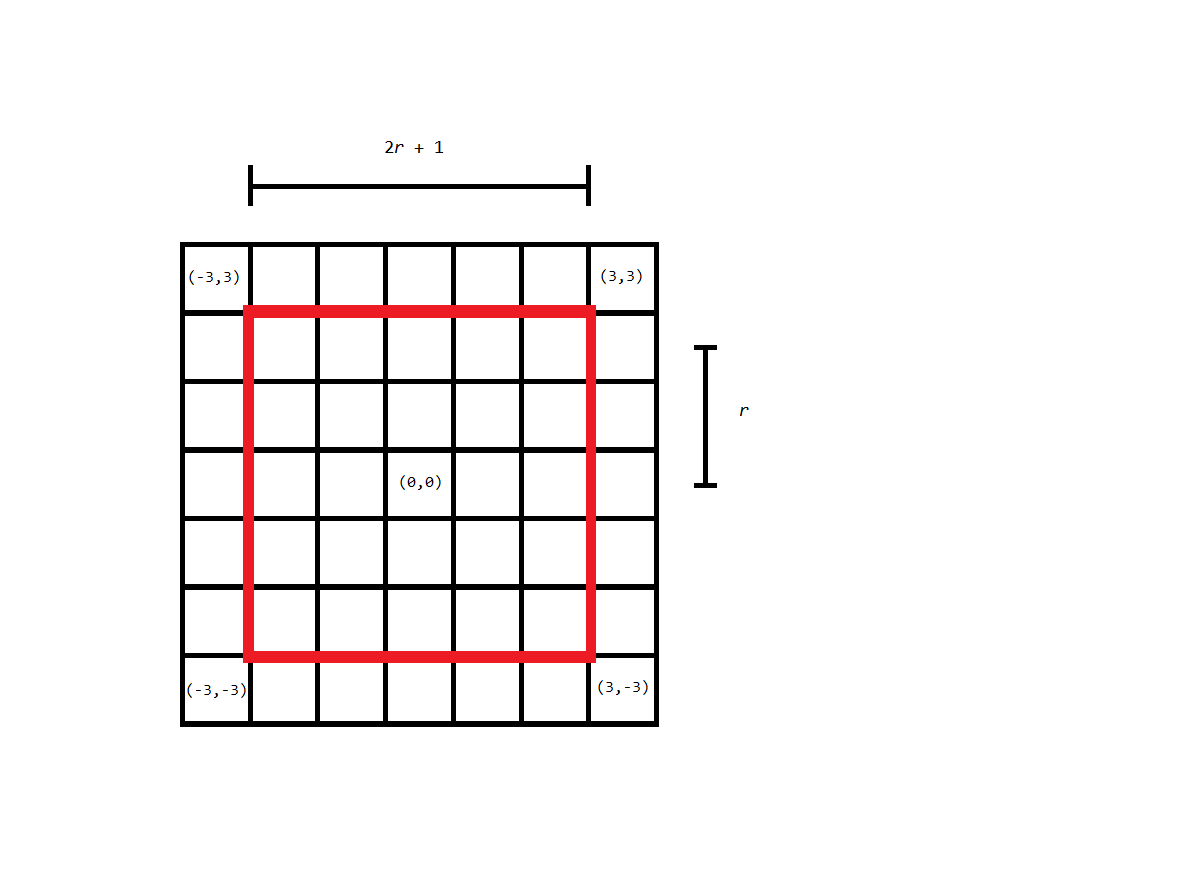
\includegraphics[width=0.9\textwidth]{tilemap}
\par\end{centering}

\caption{Illustrating a $7\times7$ tile map. The tiles inside the red zone
are being queried by specifying the tile at $(0,0)$ and the range
$r=2$\label{fig:TileWorldIlustrationInTileExtension}}


\end{figure}


This extension represents the world as a two-dimensional array of
tiles using what we will call a tile map( as can be seen in fig. \ref{fig:TileWorldIlustrationInTileExtension}).\emph{
}Tiles in this sense are squares that fit exactly one entity. We have
implemented it so that the tile in the center has the position $(0,0)$.
This means that all positions are given relative to the origo tile
at $(0,0)$. As a consequence of this, a tile map must have odd dimensions,
as it would otherwise not have a center tile. If the user tries to
access a tile that is out of bounds (for example the tile at position
$(0,n+1)$ in a $n\times n$ tile map), a tile containing a special
entity signaling that the tile is not part of the world is returned.
This ensures that querying the tile map for a tile at any position
will never fail and always return a valid value. As well as accessing
tiles at arbitrary positions, the tile map can be queried with a position
and a range $r$, in which case a two dimensional array of size $(2r+1)\times(2r+1)$
is returned, containing the tiles in that square (see fig. \ref{fig:TileWorldIlustrationInTileExtension}).
This can be used when the querying of large pieces of the map at a
time is needed. When determinining an agent's vision (described below),
we use this functionality to collect all tiles in the agent's visible
range and then filter out the obscured tiles.

In the tile extension, we have provided several modules that can be
equipped to agents to make them better suited for inhabiting a tile
based environment. For example, the \emph{movement blocking-} and
\emph{vision blocking} modules apply to all entities with a physical
presence in the environment; given another entity, they specify whether
the entity they are attached to blocks the aforementioned entity's
movement or vision, respectively. 

Also provided in the Tile Extension is a \texttt{MoveUnit }action
which is designed to move agents along a vector inside the Tile world.
This action requires a \emph{speed} module, defining how long it takes
for an agent to move one tile.


\subsubsection*{Vision}

The tile extension also provides means for seeing tiles around an
entity via the \texttt{Vision} module. All entities that are able
to sense their surroundings also have a \texttt{VisionRange} module
which -- as the name implies -- defines how far (in tiles) the entity
can see.

When the vision module is asked to return its percepts, it asks the
world to build it a \texttt{Vision} object, which it returns. The
\texttt{Vision} object uses an algorithm described in sec. \ref{sub:ImplementationTileExtension}
to assemble a set of mappings from positions (relative to the entity)
to tile references. 


\subsection{EIS Extension\label{sub:EIS-Extension}}

The EIS extension provides means for communicating with an EIS instance
over a socket, as well as serializing and deserializing percepts and
actions encoded in an XML representation of EIS'\texttt{ }IILang format.
The extension features a custom agent controller and manager, which
have been developed to work with EIS. 

As EIS is implemented in Java and our engine is written in C\#, information
can not easily be passed between the two in a native manner. Instead,
we have opted to have them communicate over sockets. As EIS already
supports formatting IILang objects to XML, we chose this to encode
information passed over the sockets. We have implemented our own IILang
object tree in C\#, which implements XML serialization and deserialization,
as well as a Java class used to parse XML to IILang objects. 

Furthermore, we have implemented special package streaming objects
in both C\# and Java, which sends the size of a payload before the
actual data when streaming XML over sockets. This allows us to detect
when an XML message has been completely received. This means that
designers wanting to use EIS with our engine should implement our
accompanying Java libraries, as well as the EIS engine extension.

In order for an EIS instance to connect to an agent controller, it
must connect to a socket which is known by both the EIS instance and
the engine at runtime. The agent manager listens to this socket and
accepts the connection. As the EIS instance connects, it receives
a new socket which can be used to communicate with the agent controller.
It now sends an XML message with the name of the agent on this socket,
and the agent manager constructs an agent controller tied to this
name and socket. The controller and the EIS instance now have their
own private socket connection to communicate on, and the agent manager
proceeds to listen for other APL instances requesting an agent controller.


\subsubsection*{Execution Protocol}

The EIS instance can now proceed to send actions to be executed by
the agent controller. When such an action is received, the controller
enqueues it, and sleeps till it is finished, at which point it resumes
listening for actions on the socket. The request to return all percepts
is just an action with the name \texttt{getAllPercepts}, which causes
the controller to gather all available percepts from the attached
agent and sent them to the EIS instance via the socket. Note that
by default, this is the only way perepts are sent; percepts are returned
in response to no other actions. Since the agent controller effectively
blocks on actions, the EIS instance can not have the controller queue
other actions or return percepts when it is executing an action that
takes time, such as the tile extension's move action (this is a restriction
imposed by the agent controller base class as described in section
\ref{sec:SystemFeaturesAgentControllers}, as it is the default behaviour
of the \texttt{performAction} method).


\paragraph*{Problems With the Chosen Execution Protocol}

The execution sequence deescribed above is very simple, but has some
downsides. Consider, for example, that two agents wish to communicate
with each other through the engine via a \texttt{talk} action. It
could be that agent $a_{1}$ wanted to ask agent $a_{2}$ whether
a certain tile was a desirable place to go. In that case, $a_{1}$'s
APL would have the action queued in the engine, which would execute
it and place the question in $a_{2}$'s mailbox. If, however, $a_{2}$
had just started a lenghty action, such as moving, its APL would not
get notified that it had been asked a question until the move was
complete, and the controller could respond to the \texttt{getAllPercepts}
action. This introduces quite some delay in performing such actions,
which are rather important in a multi-agent system. 

To remedy this, the system could be designed such that the controller
instead blocked on the call to return all percepts until the agent
had some new percepts available. In the communication example described
above, $a_{2}$ would immediately perceive that $a_{1}$ had asked
it a question, which would cause its controller to send all $a_{2}$'s
percepts (including the question) to the waiting EIS instance. Assuming
that the corresponding AP prioritizes answering the question, $a_{1}$
would have its answer in the shortest possible amount of time. In
general, allowing agents to perform multiple actions at the same time
makes the world more responsible in a number of ways. As another example,
agents in a tile based world (or any world that allows vision) could
subscribe to events on tiles they could see, and be able to respond
when eg. an enemy moved into one of them. This would allow them to
communicate the offenders position to nearby agents, or simply give
the AP a chance to preemptively figure out what the best possible
action would be to execute next.

This method does have some problems. How, for example, does $a_{2}$'s
AP know that it should prioritize answering the question, and not,
say, command the agent to begin a new move action? Since $a_{2}$
is already in the middle of a move, it would most likely break the
rules of the environment. To remedy this, the agents need to return
the action(s) they are currently executing as percepts, and the AP
would have to consider these when choosing actions. For larger environments
and agent programs, this would complicate the agent logic and percept
pool.


\subsection{Logger Extension}

One of the extensions that we provide with the engine is a simple
logger, this logger is implemented as a view on the engine and it
is meant to be used by others to add a logger for their environment.

To use the logger all that is required is that the user extends the
class \texttt{LoggerView}. The logger will then provide the extending
class with a \texttt{ThreadSafeEventManager}, which will have its
events automatically executed. As such, the only thing required by
the user is to create a \texttt{ThreadSafeEventQueue }and register
the triggers with the events the user wishes to log. 

The \texttt{LoggerView} is constructed with a \texttt{Logger} object,
on which the user can call the method \texttt{LogStringWithTimeStamp},
providing a string to be logged as well as the importance of the event,
that is, what debug level it is on. The \texttt{Logger} class is instantiated
with a maximum debug level, and will not log messages from events
with higher debug level. In this way, the user can specify if he only
wants critical errors, critical errors and warnings, or all information
to be logged.

The user must also provide the logger with a \texttt{StreamWriter
}object, this object can take many different forms however for logging
we recommend using it to wrap a file stream. 

For an example of how the logger is used, see appendix \ref{chap:VacuumWorldAppendix}.
This uses the logger as a view, to track the movements and action
of the vacuum cleaner in vacuum world.
